\section{Robot Vision Using a Pi Camera and OpenCV}
\label{robot_vision_using_pi_camera_opencv}

Giving a robot the ability to see things allows it to behave in ways to which humans relate
well. Computer vision is an area that much research is currently devoted to, but some of the
basics are already available for use in our own code, with the Pi Camera and a little bit of
work. In this section, we will use the robot and camera to drive to objects.

\begin{itemize}
\item Setting up a Raspberry Pi Camera on your robot, in terms of both software and hardware
\item Use Flask to create a web server to see what the robot sees on our laptop
\item Revisiting color models and learning how to mask images with them.
\item Using contours to detect the largest blob of color in an image and pointing the robot at it
\item Using Haar cascades to detect faces, and pointing the pan-and-tilt mechanism at them
\end{itemize}

\subsection{Set up the Raspberry Pi Camera}
We will first attach the camera to the pan-and-tilt assembly. We can then use a longer cable
to wire the camera into the Pi.

\subsection{Wire the Camera}
\label{wire_the_camera}

The Raspberry Pi has a slot specifically for the camera, the camera cable fits into this, see Figure \ref{raspberrypi_hdmi_csi}. We will be wiring our camera into this slot.

\begin{figure}[!htb]
\begin{center}
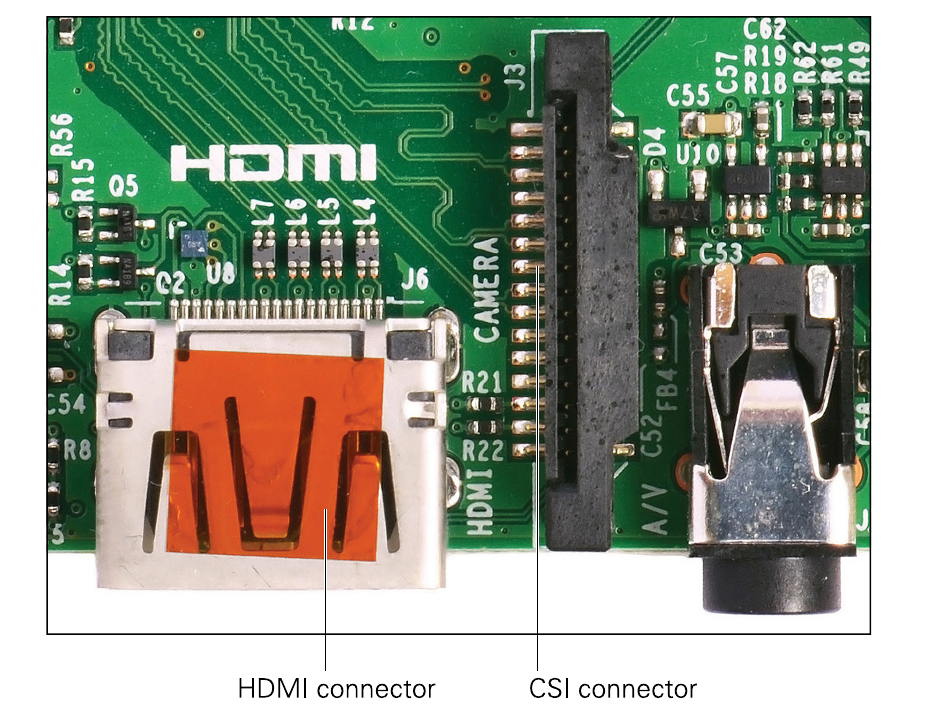
\includegraphics[scale=0.280]{img/raspberrypi/raspberrypi_hdmi_csi.jpeg}
\end{center}
\caption{ CSI and HDMI connectors.}
\label{raspberrypi_hdmi_csi}
\end{figure}

\begin{framed}
\begin{remark}{\textbf{Troubleshoot}}


See 

\url{https:/​/​www.​techcoil.​com/​blog/​connect-​raspberry-​pi-​camera-​module-​raspberry-​pi-2-​raspberry-​pi-​3/}
on how to connect the raspberry pi camera module using the long 300 mm cable. 
\end{remark}
\end{framed}

\subsection{Activate the Camera}
\label{activate_camera}

In this section, we will set up the camera, activating it in Raspbian and getting a test
picture. 

Power up the Pi on external power (that is, plugged into a USB wall adapter) for this
operation,  and log in via PuTTY. At the Terminal, type the following:

\begin{lstlisting}
sudo raspi-config
\end{lstlisting}

In \lstinline{raspi-config}, select the \textbf{5 Interfacing Options} option,and then select P1 Camera. 
You will then be asked if you would like the camera interface to be enabled. Select Yes and Ok, then Finish. 
If you are asked to reboot at this point, answer Yes. 


\subsubsection{Get a Picture from the Pi}
\label{get_a_picture}

Now that we enbled the camera, the first thing we need to do, is to confirm that our setup was successful.
Thus, we will use the Pi camera to take a picture for us. This will check whether all the connections are good or not.
If there are problems detecting the camera, please go back and check that the cable
connection is correct, that you have installed picamera, and that you have enabled the
Raspberry Pi camera in \lstinline{raspi-config}.

Reconnect to the Raspberry Pi with PuTTY, and type the following to get a picture:

\begin{lstlisting}
raspistill -o test.jpg
\end{lstlisting}

\lstinline{raspistill} takes a still image, and the \lstinline{-o} parameter tells it to store that image in
\lstinline{test.jpg}. 

We can use the FileZilla client (see appendix) to download this image and verify it on our computer. 


\subsection{Setting up OpenCV}
\label{setup_opencv}

\subsection{Install OpenCV}


\begin{framed}
\begin{remark}

Have a look at the following links should you have problems in setting up OpenCV in Raspberry Pi
\url{https://blog.piwheels.org/how-to-work-out-the-missing-dependencies-for-a-python-package/}
\end{remark}
\end{framed}

%\subsection{Access the RaspberryPi Camera}


%If we use Python we should install the \lstinline{picamera} library. This can be done via

%\begin{lstlisting}
%sudo apt-get install python-picamera python3-picamera python-rpi.gpio.
%\end{lstlisting}


%\begin{framed}
%\theoremstyle{remark}
%\begin{remark}{}

%ValueError: Unable to determine if this system is a Raspberry Pi
%\end{remark}
%\end{framed}

%The camera connects to the Raspberry Pi by installing it into the connector marked
%camera on the Raspberry Pi. To see how this is to be done, see the video at 
%\begin{lstlisting}
%http://www.raspberrypi.org/help/camera-module-setup/.
%\end{lstlisting}



